\documentclass[12pt]{article}

\usepackage[a4paper,left=3cm,top=3cm,right=2cm,bottom=2cm]{geometry}

\usepackage[utf8]{inputenc}
\usepackage[T1]{fontenc}
\usepackage[brazil]{babel}
\usepackage{newtxtext,newtxmath}
\usepackage{indentfirst}
\usepackage{setspace}
\usepackage{titlesec}
\usepackage{graphicx}
\usepackage{float}
\usepackage{enumitem}
\usepackage{hyperref}

\usepackage{fancyhdr}
\pagestyle{fancy}
\renewcommand{\headrulewidth}{0pt}
\fancyhf{}
\fancyhead[rh]{\thepage}
\fancypagestyle{plain}{
  \renewcommand{\headrulewidth}{0pt}
  \fancyhf{}
  \fancyhead[rh]{\thepage}
}
\setlength{\headheight}{15pt}

\makeatletter
\def\verbatim@font{\small\ttfamily}
\makeatother

% Configuracoes ABNT %
\onehalfspacing{}
\setlength{\parskip}{6pt}
\setlength{\parindent}{1.5cm}
\titlespacing{\section}{0pt}{12pt plus 4pt minus 4pt}{12pt plus 4pt minus 4pt}

\begin{document}

\title{Guia Rápido para Simulação Utilizando o ModelSim}

\author{Laboratório de Robótica da UFBA}

\date{2021}

\maketitle

\setcounter{page}{1} % needed if pages are to be continuously numbered

\section{Carregando Arquivos no ModelSim}
Para simular seu módulo compilado no Quartus é necessário carregar tanto ele quanto um arquivo de test bench contendo os casos de teste no ModelSim.

\begin{enumerate}[font=\bfseries]
    \item Crie uma pasta contendo seus arquivos de módulo e test bench, caso ainda não exista.

    \item Inicie o ModelSim pelo menu de aplicativos.
    \begin{figure}[H]
    \centering
    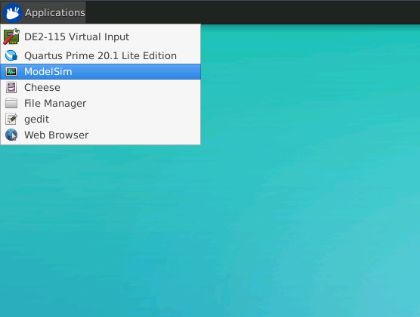
\includegraphics[width=0.6\textwidth]{img/modelsim_open.jpg}
    \caption{\label{ref:modelsim-open}Atalho para o ModelSim.}
    \end{figure}

    \pagebreak

    \item Crie um novo projeto navegando em \textit{File->New->Project}, e confirmando o nome e local dos arquivos.
    \begin{figure}[H]
    \centering
    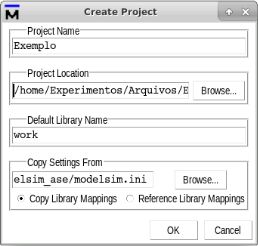
\includegraphics[width=0.5\textwidth]{img/modelsim_project.jpg}
    \caption{\label{ref:modelsim-project}Criação de novo projeto.}
    \end{figure}

    \item Na nova janela que abriu, clique em \textit{Add Existing File}, selecione os arquivos do módulo e test bench e clique em \textit{OK.}
    \begin{figure}[H]
    \centering
    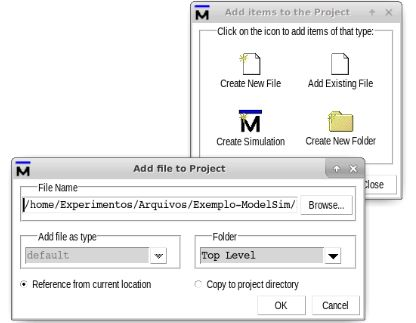
\includegraphics[width=0.7\textwidth]{img/modelsim-add-files.jpg}
    \caption{\label{ref:modelsim-add-files}Seleção de arquivos do projeto.}
    \end{figure}

    \pagebreak

    \item Compile os arquivos pelo menu \textit{Compile->Compile All} e observe se foram compilados com sucesso pelo sinal verde ao lado dos arquivos e texto de confirmação no console.
    \begin{figure}[H]
    \centering
    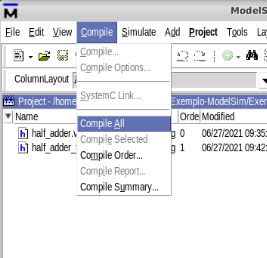
\includegraphics[width=0.5\textwidth]{img/modelsim-compile.jpg}
    \caption{\label{ref:modelsim-compile}Menu de compilação.}
    \end{figure}
    
\end{enumerate}
Feito isso o projeto está pronto para ser simulado.

\section{Simulação e Análise do Waveform}
Com os arquivos compilados no ModelSim a simulação pode ser iniciada.

\begin{enumerate}[font=\bfseries]
    \item Navegue pelo menu \textit{Simulate->Start Simulation} e na nova janela expanda o item \textit{work}, selecione o arquivo de test bench e clique em \textit{OK}.
    \begin{figure}[H]
    \centering
    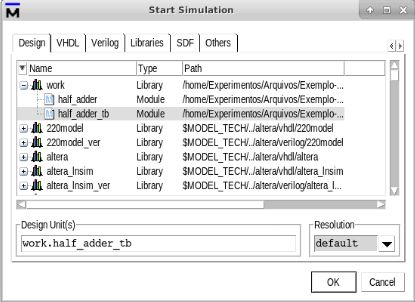
\includegraphics[width=0.6\textwidth]{img/modelsim-simulate.jpg}
    \caption{\label{ref:modelsim-simulate}Seleção de arquivo para simular.}
    \end{figure}

    \item Para abrir o waveform clique com o botão direito na instância do test bench na janela principal, e selecione a opção \textit{Add Wave.}
    \begin{figure}[H]
    \centering
    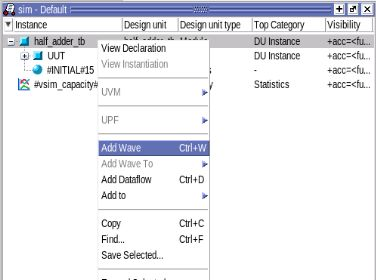
\includegraphics[width=0.6\textwidth]{img/modelsim-waveform.jpg}
    \caption{\label{ref:modelsim-waveform}Abrindo waveform do test bench.}
    \end{figure}

    \item Para melhor visualização a janela de waveform pode ser descolada da janela do ModelSim clicando no botão de \textit{Dock/Undock} no canto superior direito da janela (o do meio).
    \begin{figure}[H]
    \centering
    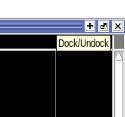
\includegraphics[width=0.3\textwidth]{img/modelsim-undocking.jpg}
    \caption{\label{ref:modelsim-undock}Undocking do waveform.}
    \end{figure}

    \item É possível adicionar variáveis à janela de waveform para monitoramento. Basta clicar com o botão direito na variável desejada na janela de \textit{Objects} no ModelSim e selecionar a opção \textit{Add Wave}.
    \begin{figure}[H]
    \centering
    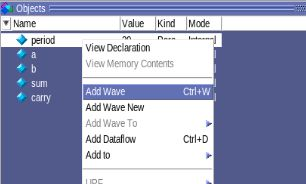
\includegraphics[width=0.6\textwidth]{img/modelsim-object.jpg}
    \caption{\label{ref:modelsim-object}Adição de objetos ao waveform.}
    \end{figure}

    \item Para iniciar a simulação do waveform basta preencher o tempo total de execução na caixa em meio aos ícones da janela \textit{Wave} e clicar no botão ao lado com um ícone de papel com seta apontando para baixo. 
    \begin{figure}[H]
    \centering
    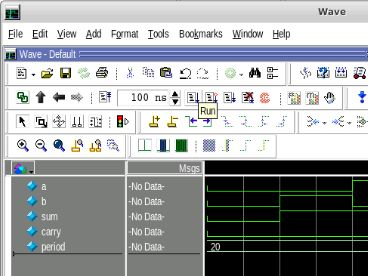
\includegraphics[width=0.8\textwidth]{img/modelsim-runwave.jpg}
    \caption{\label{ref:modelsim-runwave}Tempo de execução e botão \textit{Run} do waveform.}
    \end{figure}
\end{enumerate}

Gerado o waveform o usuário pode navegar pela linha do tempo e observar a variação no estado das variáveis. A visualização pode ser modificada pelas diversas opções presentes na janela e nos menus de botão direito em cada variável.

\end{document}
